\section{Evaluation}
The experiental results are presented and analyzed in this section.
In detail, experimental settings are introduced in Sec.~\ref{sec:experiment-settings}.
Sec.~\ref{sec:experiment-e2e}-Sec.~\ref{sec:experiment-case-study} conduct the experiments.

\begin{table}[h]
    \centering
    \begin{tabular}{c|c|c|c}
    \hline
    Dataset & |V| & |E| & Disk Space Usage\\ 
    \hline
    $G_{sf10}$& 29,987,835 & 88,317,856 & 8.9G \\
    \hline
    $G_{sf30}$ & 88,789,833 & 278,652,443 & 28.0G\\
    \hline
    $IMDB$ & 14,431,946 & 59,758,241 & 3.7G \\
    \hline
    \end{tabular}
    \caption{Statistics of the datasets. In detail, $|\cdot|$ represents the number of elements in $\cdot$.}
    \label{table:experiment-datasets}
\end{table}

\subsection{Expermental Settings}
\label{sec:experiment-settings}

\textbf{Benchmarks.} In the experiments, two commonly-used benchmarks are leveraged.
The first is the Linked Data Benchmark Council Social Network Benchmark (abbr.~LDBC-SNB or SNB).
For this benchmark, two datasets, i.e., $G_{sf10}$ and $G_{sf30}$ generated with scale factor 10 and 30 respectively, are utilized.
These datasets are mainly about the relationships among persons, forums, posts, comments, locations, and tags.
The queries performed on these datasets are from the LDBC Interactive Complex workloads.
Since we focus on the proving the superiority of the converged optimizer compared to the existing optimzers, we simplify the queries and modify the queries following the experiments of GrainDB \cite{graindb}.
That is, queries IC-10, IC-13, and IC-14 are dropped, and queries containing variable-length joins are broken down into several individual queries, with each one featuring a join along a path with a fixed length.
Specifically, IC-5-2 represents a query obtained by modifying IC-5, and 2 is th length of the path.
The obtained modified benchmark is denoted by SNB-M and queries performed on $G_{sf10}$ and $G_{sf30}$ are from SNB-M.

The other benchmark is Join Order Benchmark (JOB) on Internet Movie Database (abbr.~IMDB).
Specifically, IMDB is a dataset mainly about the relationships among movies, persons, and movie companies.
JOB focuses on the problem of join order optimization, and queries in JOB have an average of 8 joins.
The details of the datasets are summarized in Table \ref{table:experiment-datasets}, where |V| and |E| represent the number of vertices and edges in the datasets, respectively.
For IMDB, its tables are regarded as vertices or edges first, and then the number of vertices and edges are counted.

\textbf{Baselines. }
In the experiments, two optimizers of type $Rel$ and $Rel^+$ respectively are utilized as the baselines.
Specifically, the opitmizer of type $Rel$ is that of DuckDB, which is a well-known open-source database.
The version of DuckDB is 0.9.2.
The optimizer of type $Rel^+$ is that of GrainDB.
It optimizes queries with the optimizer of DuckDB first, and then replaces some hash joins in the obtained physical plans with sip joins or merge sip joins.
To ensure the fairness of the comparison, we first upgrade the version of DuckDB that is integrated into GrainDB to 0.9.2.
Then, given a query, after a physical plan w.r.t.~this query is obtained by an optimizer, the plan is transformed to that of GrainDB.
Therefore, different plans can be executed by the the backend, and the efficiency of the plans obtained by varied optimizers can be compared fairly.
Please note that codegen techniques can be employed to facilitate the transformation of the physical plan.
For simplicity, in the rest of this paper, when there is no ambiguity, the optimizers of DuckDB and GrainDB are shortened to DuckDB and GrainDB, respectively.

Our experiments are carried out on a server with Intel Xeon E5-2682 2.50GHz CPU and 251GB RAM.

\subsection{End-to-End Experiments}
\label{sec:experiment-e2e}

on LDBC SNB sf-10, sf-30
on IMDB Job

\subsection{Queries with Circles}
\label{sec:experiment-circle}

1. Source - ExpandE - ExpandV (sip) v.s. Source - ExpandV (mergesip)

2. intersect v.s. join twice


\subsection{Ablation Study}
\label{sec:experiment-ablation}

remove graph index (i.e., duckdb)
remove extend-intersect


\subsection{Detailed Evaluation}
\label{sec:experiment-detail}

time cost of index building
compilation
query execution

\subsection{Optimization Efficiency Evaluation}
\label{sec:experiment-optimize}

In this subsection, experiments are conducted to compare the optimization time cost of relgo and Apache Calcite, which is a well-known data management framework widely used in various projects such as Hive and Kylin.
Please note that the codes of relgo and Calcite are both written in Java.
In detail, we test the optimization time of relgo and Calcite on SNB-M and JOB benchmarks, and VolcanoPlanner of Calcite with default rules is leveraged.
If optimization for a query is not finished in 10 minutes, the process is early stopped and the time cost of such optimization is recorded as 10 minutes.
The results are shown in Fig.~\ref{fig:exp-optimization}.

\begin{figure*}
    \centering
    \begin{subfigure}[b]{0.3\linewidth}
        \centering
        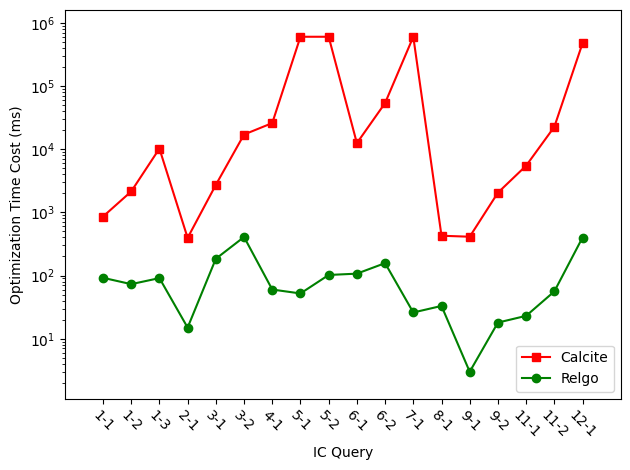
\includegraphics[width=\linewidth]{./figures/exp/optimization_sf10.png}
        \caption{Optimization Time Cost on $G_{sf10}$.}
        \label{fig:exp-optimization-sf10}
    \end{subfigure}
    \begin{subfigure}[b]{0.3\linewidth}
        \centering
        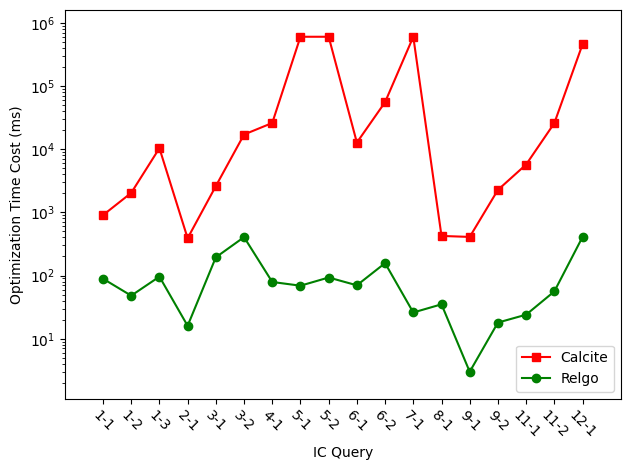
\includegraphics[width=\linewidth]{./figures/exp/optimization_sf30.png}
        \caption{Optimization Time Cost on $G_{sf30}$.}
        \label{fig:exp-optimization-sf30}
    \end{subfigure}
    \begin{subfigure}[b]{0.3\linewidth}
        \centering
        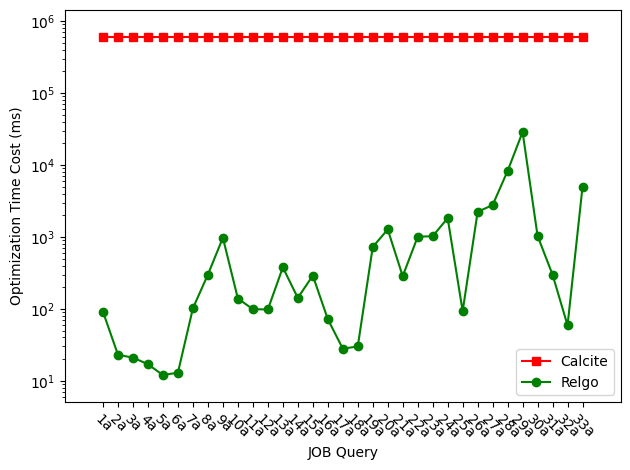
\includegraphics[width=\linewidth]{./figures/exp/optimization_job.png}
        \caption{Optimization Time Cost on JOB.}
        \label{fig:exp-optimization-job}
    \end{subfigure}
    \caption{Experiments on the time cost of optimization.}
    \label{fig:exp-optimization}
\end{figure*}

In the experiments, optimizing all the queries with relgo can be finished in 10 minutes, while optimizing some queries with Calcite exceeds the 10-minute limit.
For example, when JOB benchmark is utilized, the time cost of optimizing all the queries with Calcite is longer than 10 minutes.
As shown in Fig.~\ref{fig:exp-optimization}, relgo is much more efficient than Calcite in optimizing queries, and it is consistent with the conclusions obtained in Sec.~\ref{sec:theoretical-analysis}.
For instance, when IC5-1 is queried on $G_{sf30}$, the time cost of query optimization with relgo can be more than $10^4\times$ faster than that of Calcite.

Besides, the optimization time cost of relgo is similar on $G_{sf10}$ and $G_{sf30}$, and so is Calcite.
The reason is that the time required for optimization is not significantly associated with the scale of the dataset; instead, it is related to the relative cardinalities among the different tables.
The relative cardinalities in LDBC datasets of different scales are consistent, therefore the optimization time is similar.

\begin{figure}
    \centering
    \begin{subfigure}[b]{.3\linewidth}
        \centering
        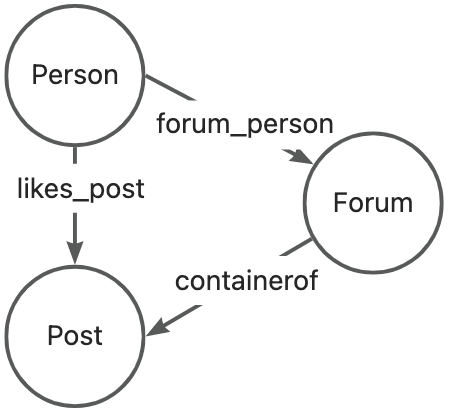
\includegraphics[width=\linewidth]{./figures/exp/pattern-triangle.png}
        \caption{Triangle}
        \label{fig:exp-hard-triangle}
    \end{subfigure}
    \begin{subfigure}[b]{.3\linewidth}
        \centering
        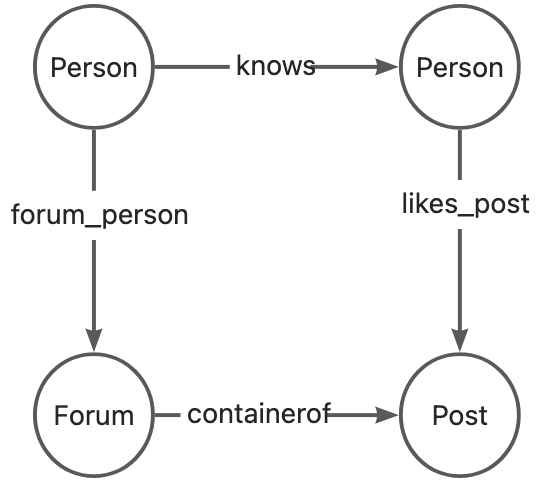
\includegraphics[width=\linewidth]{./figures/exp/pattern-butterfly.png}
        \caption{Butterfly}
        \label{fig:exp-hard-butterfly}
    \end{subfigure}
    \begin{subfigure}[b]{0.3\linewidth}
        \centering
        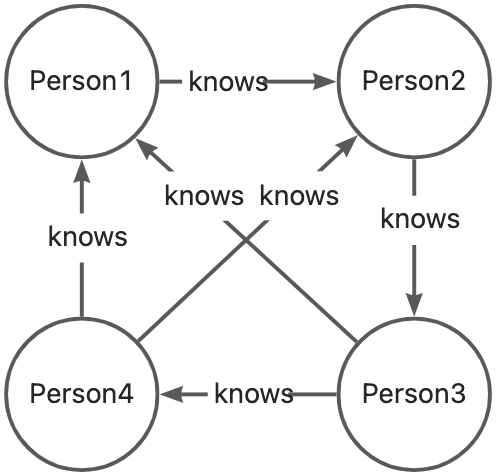
\includegraphics[width=\linewidth]{./figures/exp/pattern-clique.png}
        \caption{4-Clique}
        \label{fig:exp-hard-clique}
    \end{subfigure}
    \caption{Patterns searched for in case studies.}
    \label{fig:exp-hard-patterns}
\end{figure}

\subsection{Case Study}
\label{sec:experiment-case-study}

In this section, to highlight the strengths our converged optimizer, i.e., relgo, we design three SQL/PGQ queries to find the patterns shown in Fig.~\ref{fig:exp-hard-patterns} on $G_{sf10}$ and $G_{sf30}$.
Take finding 4-cliques as an example, the corresponding SQL/PGQ query is as follows:
\begin{lstlisting}
    SELECT pn1, pn2, pn3, pn4 
    FROM GRAPH_TABLE (knows_grpah
        MATCH (p1:Person)-[:Knows]->(p2:Person)-[:Knows]->(p3:Person)-[:Knows]->(p4:Person),
            (p4)-[:Knows]->(p1)-[:Knows]->(p3),
            (p2)-[:Knows]->(p4)
        COLUMNS (
            p1.id as pn1, p2.id as pn2, 
            p3.id as pn3, p4.id as pn4
        )
    );
\end{lstlisting}
With these three queries, the efficiency of the physical plans obtained by relgo and those obtained by GrainDB are compared.
The experimental results are shown in Fig.~\ref{fig:exp-hard}.


\begin{figure}
    \centering
    \begin{subfigure}[b]{.45\linewidth}
        \centering
        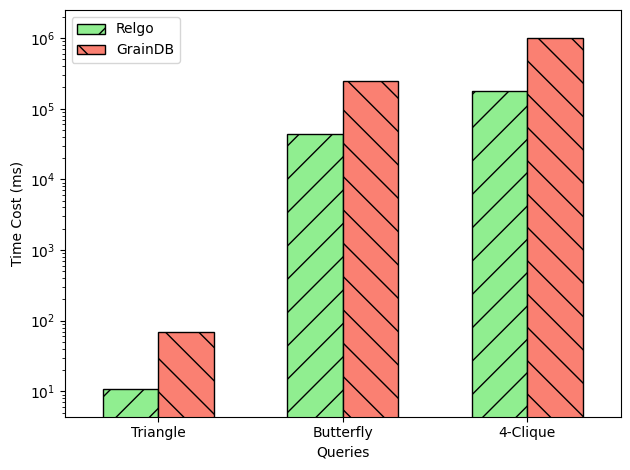
\includegraphics[width=\linewidth]{./figures/exp/hard_sf10.png}
        \caption{Time Cost on $G_{sf10}$.}
        \label{fig:exp-hard-sf10}
    \end{subfigure}
    \begin{subfigure}[b]{0.45\linewidth}
        \centering
        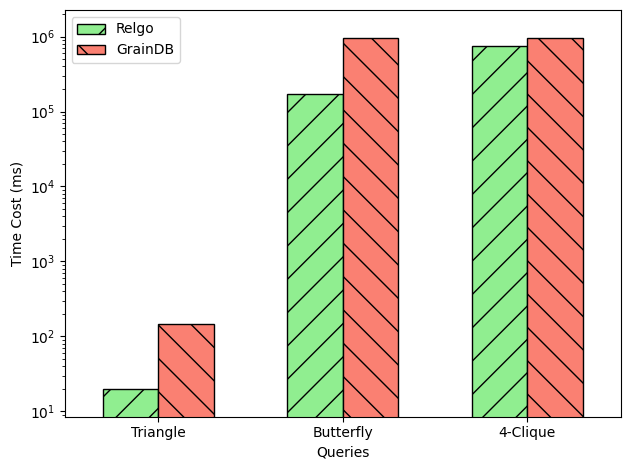
\includegraphics[width=\linewidth]{./figures/exp/hard_sf30.png}
        \caption{Time Cost on $G_{sf30}$.}
        \label{fig:exp-hard-sf30}
    \end{subfigure}
    \caption{Experiments on the time cost of finding patterns in Fig.~\ref{fig:exp-hard-patterns} on $G_{sf10}$ and $G_{sf30}$.}
    \label{fig:exp-hard}
\end{figure}

The experimental results indicate the superiority of relgo compared with GrainDB.
In detail, the physical plans obtained by relgo are always much better than those obtained by GrainDB.
Under the best conditions, i.e., the 4-clique pattern queried on $G_{sf30}$, the execution time of the plan optimized with relgo can be more than an order of magnitude shorter than that of GrainDB.
Such a significant improvement comes from relgo's more accurate estimation of cost, and a better plan can be generated.
Besides, \expandintersectrule can be utilized in the plan generated with relgo, and it is much more efficient than performing multiple joins [as illustrated in Sec.~\ref{sec:experiment-ablation}].

